%% ----------------------------------
%%   Kap01---Einleitung.tex
%% ----------------------------------

%% Welches Problem soll gelöst werden?

\chapter{Einleitung}
\label{sec:Chapter1}


Der Memristor wurde erstmals 1971 von Leon Chua in der Veröffentlichung~\cite{chua_mem} erwähnt, da dieser aus Gründen der Symmetrie zwischen dem elektrischen Strom, der Spannung, der Ladung und dem magnetischen Fluss schloss, dass es ein viertes, fundamentales, passives Schaltelement neben dem Widerstand, dem Induktor und dem Kondensator geben muss (siehe Abb.~\ref{fig:sym_mem}).

\begin{figure}
  \centering
    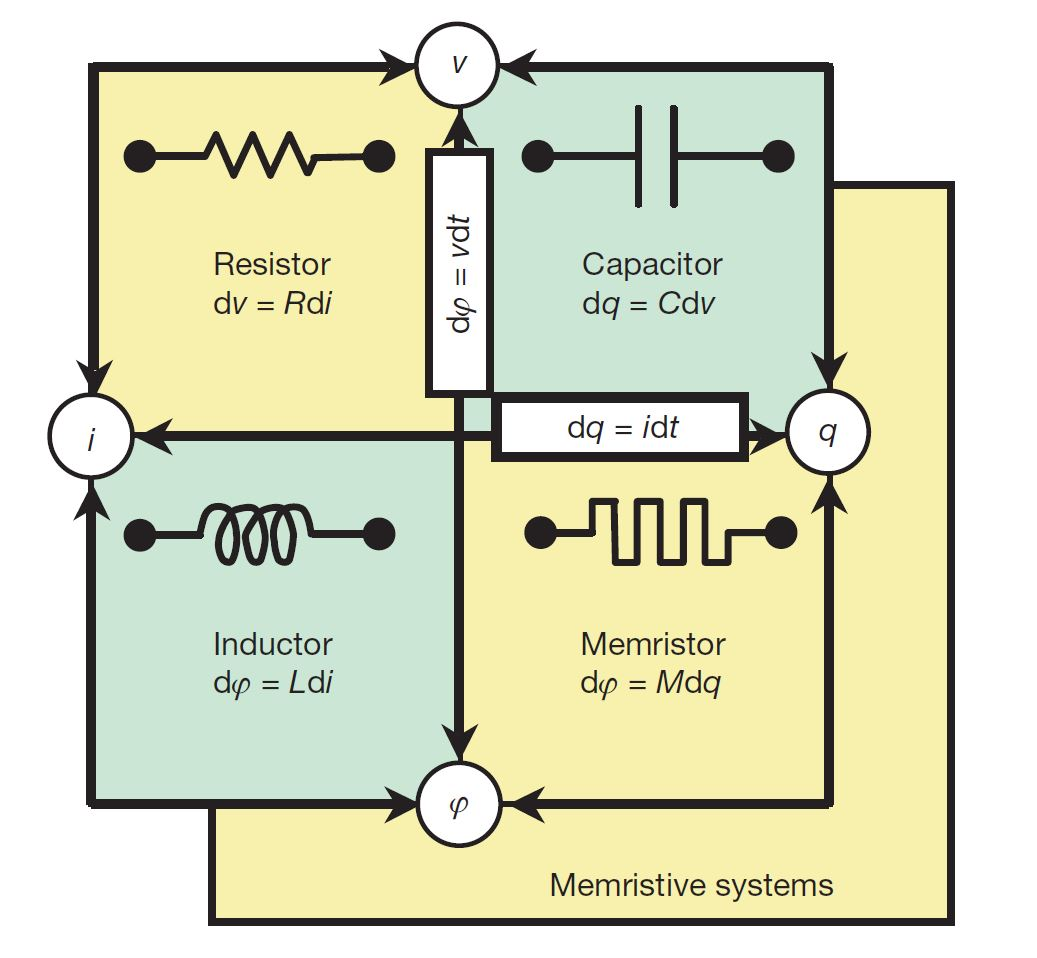
\includegraphics[width=0.6\textwidth]{images/symmetrie_memristor.JPG}
    \quelle{\cite{hp_2008}}
  \caption{Symmetrie zwischen Stromstärke i, Spannung v, Ladung q und dem magnetischen Fluss $\varphi$ , welche zur Entdeckung des Memristors führte.}
  \label{fig:sym_mem}
\end{figure}

Strukov, Snider, Stewart und Williams gelang es im Jahr 2008 den ersten funktionierenden Memristor für HP~\cite{hp_2008} zu entwickeln, obwohl Chua die Existenz eines solchen Bausteins schon 37 Jahre vorher postulierte. Das Wort \glqq Memristor\grqq, eine Wortneuschöpfung und Abkürzung für \glqq Memory Resistor\grqq, bildet allgemein einen Oberbegriff für alle Speichermedien, welche durch Widerstandsschaltungen realisiert sind. Dementsprechend gibt es nicht den einen Memristor, sondern viele verschiedene Modelle von Memristoren.

Die Entwicklung und Forschung auf dem Gebiet der Memristoren schreitet seit Jahren weiter voran. Viele Experten sind der Meinung, dass Memristoren die Speichermedien revolutionieren werden. Andere Firmen neben HP, wie Knowm Inc.~\cite{knowm_comp_2019}, produzieren Memristoren und bieten sie zum Verkauf an, um diese Schaltungselemente zu Forschungszwecken verfügbar zu machen. Doch da der Memristor noch ein relativ junges Schaltungselement darstellt, obwohl er in der Theorie schon fast 50 Jahre und in der Praxis knapp zwölf Jahre existiert, sind aktuelle Memristoren von sehr unbeständiger Qualität. Auf einem Chip von 8 bis 16 Memristoren aus der Produktion von Knowm Inc. gibt es unter den Memristoren des gleichen Materials oftmals bereits große Unterschiede in ihrer Beschaffenheit. Die Unterschiede im Material sind ein weiterer Punkt, welcher in Hinblick auf die Qualität von Memristoren betrachtet werden muss. Bislang wurden noch keine
Qualitätsmerkmale aufgestellt, um einzelne Memristoren kategorisieren und klassifizieren zu können. Diese Arbeit befasst sich mit einer solchen Kategorisierung von Memristoren.

\section{Zielsetzung}

Das Ziel dieser Arbeit ist eine vollständige Klassifikation und Kategorisierung von einzelnen Memristoren nach einem selbst erstellten Qualitätsmaß. Im Zuge dieser Arbeit soll durch das Hinzufügen einer Funktionalität in der Memristor Discovery Software von Knowm Inc. möglich sein, eine automatische Klassifizierung eines ausgewählten Memristors nach einem in dieser Arbeit vorgestellten Qualitätsmaßes durchzuführen. Dabei soll der Nutzer dieser Funktionalität verschiedene Ausgaben erhalten, welche Auskunft über die Qualität und Lebensdauer des ausgewählten Memristors bieten. Das Qualitätsmaß wird außerdem so allgemein gehalten, dass es auf andere Memristor-Typen angewandt werden kann, damit der Leser dieser Arbeit neben der Implementierung ein grundlegendes Verständis über Memristoren und deren Qualitätsmerkmale erhält.

\section*{Gliederung der Arbeit}
\label{sec:Sec1.2}
Die Arbeit beginnt mit den Grundlagen in Kapitel~\ref{sec:Chapter2}. Dabei wird ein allgemeiner Überblick über Memristoren gegeben und eine Darstellung von wissenschaftlichen Arbeiten geliefert, welche Ähnlichkeiten mit dieser Arbeit besitzen oder einen Einfluss auf diese haben.

Darauf folgt das Kapitel~\ref{sec:Chapter3}, in welchem ein grundlegendes Konzept dieser Arbeit vorgestellt wird. Dabei werden die wichtigsten Qualitätsmerkmale für Memristoren definiert. Die Merkmale sind die Formbarkeit, die Speichergröße, der Energieverbrauch und die Lebensdauer. Des weiteren wird in diesem Kapitel über theoretische Ansätze zur Kategorisierung und Klassifikation der Qualitätsmerkmale diskutiert.

Das Kapitel~\ref{sec:Chapter4} liefert danach die Realisierung zum davor gelieferten Konzept und thematisiert dabei, welche Funktionalitäten aus dem Konzept in der Implementierung aufgenommen wurden und wie diese in der Praxis funktionieren. Außerdem werden Schwierigkeiten in der Implementierung der theoretischen Modelle thematisiert.

Im Kapitel~\ref{sec:Chapter5} werden im Zuge der Arbeit aufgenommene Messergebnisse dargestellt und diskutiert. Dabei wird besonders thematisiert, welchen Einfluss bestimmte Probleme auf die Messergebnisse haben.

Zuletzt wird im Kapitel~\ref{sec:Chapter6} eine Zusammenfassung der Arbeit vorgenommen. Dabei wird thematisiert, was für weitere Arbeit und Forschung getan werden kann, um die Kategorisierung und Klassifikation von einzelnen Memristoren zu verbessern.
